%%%%%%%%%%%%%%%%%%%%%%%%%%%%%%%%%%%%%%%%%%%%%%%%%%%%%%%%%%%%%%%%%%%%%%
% Template TCC Engenharia de Software - PUC Minas
% A3: 50 nós, Rodada de Validação nas rodadas 10, 20, 30, 40 e 50.
% Substituir o .tex no Overleaf e enviar a pasta figuras/ junto.
% Manter sbc-template.sty no projeto.
%%%%%%%%%%%%%%%%%%%%%%%%%%%%%%%%%%%%%%%%%%%%%%%%%%%%%%%%%%%%%%%%%%%%%%

\documentclass[12pt]{article}

\usepackage[utf8]{inputenc}
\usepackage{sbc-template}
\usepackage{graphicx,url}
\usepackage{float}
\usepackage[brazil]{babel}
\usepackage{tabularx}
\newcolumntype{C}{>{\centering\arraybackslash}X}
\newcolumntype{L}[1]{>{\raggedright\arraybackslash}m{#1}}
\usepackage[inline]{enumitem}
\usepackage{tcolorbox}
\usepackage{amsmath}
\usepackage{tikz}
\usetikzlibrary{arrows.meta,positioning,shapes.geometric}

\sloppy
\raggedbottom

\title{Simulação de Rede Distribuída para Inferência de IA com Avaliação de Confiabilidade baseada em Reputação}

\author{Allan Mateus de Souza Arruda\inst{1}, Lara Andrade Carvalho\inst{1}}

\address{Curso de Engenharia de Software -- Pontifícia Universidade Católica de Minas Gerais (PUC Minas)\\
  Belo Horizonte -- MG -- Brasil
  \email{\{allan.arruda, lara.carvalho\}@sga.pucminas.br}
}

\begin{document}

\maketitle

\begin{abstract}
  Distributed execution of Artificial Intelligence (AI) inference can reduce dependence on a single provider, but it also exposes the aggregated result to honest errors and Byzantine behaviour. This work investigates whether a reputation mechanism changes the accuracy of redundant inference in a simulated network of 50 nodes with colluding malicious nodes. The reputation chosen here is the moving average $r \leftarrow (1-\alpha)r + \alpha s$, where $s$ comes from the weighted consensus or, on a Validation Round, from the ground truth. With a fixed orchestrator and $\alpha = 0.3$, test accuracy is $1$ up to $25\%$ malicious nodes and $0$ at $50\%$, $65\%$ and $80\%$. With a dynamic orchestrator, it is $1$ through $80\%$, also without ground truth; from $65\%$ on, the value comes from the honest nodes' copy of the record. Answers come from profiles, not from SmolLM3-3B.
\end{abstract}

\begin{resumo}
  A execução distribuída de inferência de Inteligência Artificial (IA) pode reduzir a dependência de um único provedor, mas também expõe o resultado agregado a erros honestos e a comportamento bizantino. Este trabalho investiga se um mecanismo de reputação altera a acurácia da inferência redundante em uma rede simulada de 50 nós com maliciosos em conluio. A reputação escolhida é a média móvel $r \leftarrow (1-\alpha)r + \alpha s$, em que $s$ vem do consenso ponderado ou, na Rodada de Validação, do gabarito. No orquestrador fixo, com $\alpha = 0{,}3$, a acurácia de teste é $1$ até $25\%$ de maliciosos e $0$ em $50\%$, $65\%$ e $80\%$. No orquestrador dinâmico, ela é $1$ até $80\%$, também sem gabarito; a partir de $65\%$, na cópia do registro dos nós honestos. As respostas vêm de perfis, não do SmolLM3-3B.
\end{resumo}

\begin{tcolorbox}
\footnotesize
\textbf{Bacharelado em Engenharia de \emph{Software} - PUC Minas\\
Trabalho de Conclusão de Curso (TCC)} \\

\indent Orientadora do TCC II: Isabela Borlido Barcelos \\ \\
Belo Horizonte, 11 de outubro de 2026.
\end{tcolorbox}

% -----------------------------------------------------------
\section{Introdução}

A demanda por tarefas de Inteligência Artificial (IA) motiva arquiteturas que repartem a inferência entre múltiplos participantes, para ampliar a disponibilidade e aproveitar recursos computacionais distribuídos \cite{shi2016,tanenbaum2017,coulouris2021,russell2020}. Este trabalho avalia a confiabilidade do resultado agregado quando a mesma tarefa é enviada a vários nós de uma rede distribuída e uma decisão coletiva precisa ser formada. Nesse arranjo de inferência redundante, a replicação oferece diversidade de respostas, e o mecanismo de agregação precisa lidar com falhas e com manipulação intencional.

Os participantes não escolhem a tarefa, a regra de consenso nem os vizinhos com quem trocam mensagens. O protocolo define a pergunta, a agregação e, no orquestrador dinâmico, o grafo. Os nós não são igualmente confiáveis. Um nó pode responder de forma correta na maior parte das vezes ou enviar propositalmente um valor inconsistente. O último caso corresponde a uma Falha Bizantina: um subconjunto de agentes transmite informações arbitrárias para corromper a decisão coletiva \cite{lamport1982,castro1999}. Tais falhas também afetam a fase de inferência, na qual o que se protege é a resposta devolvida, e não o vetor de parâmetros. Protocolos de acordo com autenticação criptográfica excedem o escopo deste simulador. O problema de pesquisa é: \textbf{como a reputação, atualizada pela concordância com o consenso nas rodadas normais e pelo gabarito nas Rodadas de Validação fixas, altera a acurácia do consenso em uma rede simulada de inferência redundante com 50 nós, no orquestrador fixo e no orquestrador dinâmico, diante de conluio?}

A reputação deste trabalho é uma escolha própria: a média móvel exponencial $r \leftarrow (1-\alpha)r + \alpha s$ da Equação~\ref{eq:reputacao}. No treinamento federado, cada participante treina o modelo com os próprios dados e envia só as atualizações de parâmetros. Chen et al.\ ponderam essas atualizações pelo histórico \cite{chen2024}, e o \textit{EigenTrust} usa o histórico para reduzir a influência de pares não confiáveis no compartilhamento de arquivos \cite{kamvar2003}. Nenhum desses usos protege a resposta agregada de uma inferência redundante, que é o que chega a quem fez a pergunta. Neste trabalho os nós não treinam: cada um responde à mesma pergunta e o orquestrador junta as respostas. Quem diverge do consenso perde peso, enquanto o consenso ainda for o da maioria honesta. Se um grupo em conluio passar a ser o consenso, a mesma conta aumenta o peso do grupo. A Seção~\ref{sec:resultados} mede os dois casos.

O objetivo geral é medir, em simulação, se essa reputação muda a acurácia do consenso. Os objetivos específicos são: (i)~especificar o simulador com orquestrador fixo e orquestrador dinâmico, perfis honesto e malicioso, consenso ponderado e maioria simples; (ii)~atualizar a reputação pela Equação~\ref{eq:reputacao}, com sinal de consenso nas rodadas normais, sinal de gabarito nas rodadas 10, 20, 30, 40 e 50, e calibração nas três primeiras rodadas do dinâmico com gabarito; (iii)~comparar, em 50 nós, 50 rodadas e cinco repetições, as configurações ``Fixo, com gabarito'', ``Dinâmico, com gabarito'' e ``Dinâmico, sem gabarito'', quanto à acurácia do consenso ponderado.

O restante deste documento está organizado da seguinte forma. A Seção~\ref{sec:fundamentacao} apresenta a fundamentação teórica. A Seção~\ref{sec:relacionados} discute trabalhos relacionados. A Seção~\ref{sec:metodos} descreve materiais e métodos. A Seção~\ref{sec:resultados} apresenta os resultados das 65 execuções. A Seção~\ref{sec:conclusao} sintetiza o que foi medido.

% -----------------------------------------------------------
\section{Fundamentação Teórica}
\label{sec:fundamentacao}

A literatura de sistemas distribuídos trata coordenação, falhas e consistência como problemas de projeto, independentemente de o conteúdo ser um arquivo, um log de transações ou a saída de um modelo de IA \cite{tanenbaum2017,coulouris2021}. A computação em borda motiva processar dados perto da fonte \cite{shi2016}, e revisões de IA distribuída discutem robustez, privacidade e governança \cite{wei2025,wang2025}. Neste TCC, esses conceitos situam o problema: a implementação avaliada é um simulador local, não uma implantação em dispositivos de borda.

\subsection{Inteligência Artificial Distribuída: treinamento versus inferência}

Inteligência Artificial Distribuída cobre pelo menos dois arranjos distintos. No treinamento colaborativo, os participantes enviam atualizações de parâmetros derivadas de dados locais; o servidor agrega pesos ou gradientes \cite{mcmahan2017,bonawitz2019,kairouz2021}. Na inferência redundante, adotada aqui, não há aprendizado conjunto: a mesma tarefa é submetida a vários nós e a rede devolve uma única resposta. A redundância permite medir acurácia contra um gabarito e injetar comportamento malicioso controlado. Paralelismo de camadas ou de tensores fica fora do escopo.

Falhas Bizantinas \cite{lamport1982,castro1999} aplicam-se aos dois arranjos. No treinamento, o adversário corrompe o modelo; na inferência, corrompe a resposta agregada.

Abordagens inspiradas em \textit{blockchain} para compartilhar modelos \cite{chen2024} tratam de outro objeto. Neste trabalho não há mineração nem contrato inteligente.

\subsection{Sistemas de Reputação em Redes Distribuídas}

Sistemas de reputação registram o histórico de comportamento e modulam a influência de cada participante. O \textit{EigenTrust} constrói confiança global a partir de interações locais em redes P2P \cite{kamvar2003}. Em aprendizado federado, a reputação pode ponderar atualizações maliciosas \cite{chen2024}. A reputação deste trabalho é a média móvel exponencial descrita na Seção~\ref{sec:metodos}.

% -----------------------------------------------------------
\section{Trabalhos Relacionados}
\label{sec:relacionados}

Esta seção percorre cinco temas: confiança e governança em IA distribuída (Seção~\ref{sec:eixo-ia}), aprendizado federado (Seção~\ref{sec:eixo-fl}), reputação em redes par-a-par (Seção~\ref{sec:eixo-p2p}), falhas bizantinas e consenso (Seção~\ref{sec:eixo-bft}) e conteinerização (Seção~\ref{sec:eixo-docker}). A Seção~\ref{sec:lacuna} fecha a comparação.

\subsection{Confiança e governança em IA distribuída}
\label{sec:eixo-ia}

Wei e Liu \cite{wei2025} separam a robustez na inferência, diante de evasão e de consultas irregulares, da robustez no treinamento, diante de envenenamento, ataques bizantinos e dados irregulares. Evasão e consultas irregulares não aparecem neste trabalho. O ataque medido é bizantino: um grupo devolve a mesma resposta errada, e a taxonomia deles associa esse ataque ao treinamento. Aqui ele é medido na inferência, com a mesma pergunta, vários nós e uma resposta agregada. Confiança, no argumento deles, é propriedade da arquitetura que coordena os participantes, e não um atributo isolado do modelo.

Abordagens inspiradas em \textit{blockchain} para compartilhamento de modelos \cite{blockchainAI2024} deslocam a garantia para armazenamento imutável e validação criptográfica. O livro do orquestrador dinâmico encadeia o \textit{hash} de cada rodada para que uma réplica reconheça um registro alterado. Não há mineração nem contrato inteligente.

\subsection{Aprendizado federado: o contraste}
\label{sec:eixo-fl}

McMahan et al. \cite{mcmahan2017} propõem o \textit{Federated Averaging} e mostram, no resumo do artigo, uma redução de 10 a 100 vezes no número de rodadas de comunicação em relação ao gradiente descendente síncrono. Bonawitz et al. \cite{bonawitz2019} descrevem o projeto de um sistema de aprendizado federado em produção para dispositivos móveis. Kairouz et al. \cite{kairouz2021} reúnem os avanços da área e uma coleção de problemas em aberto. Wang et al. \cite{wang2025} propõem um aprendizado federado assíncrono e descentralizado para dispositivos de borda, e o resumo do artigo relata melhor desempenho de teste com a velocidade de convergência preservada. O que esses trabalhos protegem é o vetor de parâmetros. Eles não avaliam inferência redundante, na qual a agregação ocorre sobre respostas comparáveis a um gabarito. Reutiliza-se a coordenação de participantes autônomos, e a métrica passa a ser a acurácia da resposta agregada.

Chen et al. \cite{chen2024} aplicam reputação para mitigar atualizações maliciosas em aprendizado federado assíncrono associado a \textit{blockchain}. A ponderação pelo histórico, reaproveitada aqui sobre respostas e não sobre parâmetros, vem desse trabalho. O vínculo com a atualização de modelo não é reproduzido.

\subsection{Reputação em redes par-a-par}
\label{sec:eixo-p2p}

O \textit{EigenTrust} \cite{kamvar2003} constrói uma medida de confiança global a partir de interações locais, propaga essa confiança sobre uma matriz e ancora o cálculo em participantes previamente confiáveis. O algoritmo mostra que histórico local, agregado adequadamente, pode reduzir a influência de pares que distribuem conteúdo inautêntico. Foi concebido para compartilhamento de arquivos, com avaliação binária de cada transação, e pressupõe uma rede par-a-par. A arquitetura fixa deste trabalho é uma estrela, e a dinâmica é um grafo 4-regular; nos dois casos a reputação usada no consenso é global. O mecanismo adapta a ideia de guardar o histórico na forma da Equação~\ref{eq:reputacao}. Não se calcula matriz de confiança transitiva nem se adotam nós previamente confiáveis.

\subsection{Falhas bizantinas e consenso}
\label{sec:eixo-bft}

Lamport et al. \cite{lamport1982} mostram que, sem mensagens assinadas, o acordo entre $n$ participantes, com até $f$ faltosos, exige $n \geq 3f+1$. Castro e Liskov \cite{castro1999} descrevem o PBFT (\textit{Practical Byzantine Fault Tolerance}), que chega ao acordo dentro desse limite: as réplicas trocam mensagens em fases, o líder ordena os pedidos e as demais confirmam, de modo que o serviço continua enquanto no máximo $f$ réplicas, em $n \geq 3f+1$, se comportam de forma arbitrária. Wu et al. \cite{wu2024} sistematizam a evolução desses protocolos. Bouhata et al. \cite{bouhata2025} revisam a tolerância bizantina em aprendizado de máquina distribuído, com ênfase em treinamento. O mecanismo avaliado aqui não adota o PBFT porque a pergunta é o peso que a reputação dá a cada voto, e não o acordo entre réplicas de um mesmo serviço.

\subsection{Conteinerização de ambientes experimentais}
\label{sec:eixo-docker}

Conteinerização isola um programa com as dependências e a configuração de que ele precisa para rodar do mesmo jeito em outra máquina \cite{docker2026,burns2022}. O repositório adota esse isolamento: há um \texttt{Dockerfile} e um servidor HTTP por nó, para que cada nó possa ser um processo separado. Os números da Seção~\ref{sec:resultados} foram obtidos em uma execução em processo, com os mesmos perfis e sem troca de mensagens em rede.
% PENDENTE: a razão de não usar Docker na Seção 5. A correção da A2 registrava o experimento em ambiente Docker.

\subsection{Síntese da lacuna}
\label{sec:lacuna}

Parte da literatura discute confiança em IA distribuída; outra parte aplica reputação ao treinamento federado; uma terceira formaliza consenso sob falhas arbitrárias para réplicas de serviço. A lacuna abordada é medir, em simulação controlada, se a reputação com Rodada de Validação em rodadas fixas altera a acurácia da inferência redundante, no orquestrador fixo e no dinâmico.

% -----------------------------------------------------------
\section{Materiais e Métodos}
\label{sec:metodos}

O objetivo é medir se a reputação muda a acurácia do consenso em uma rede simulada de 50 nós. As subseções seguintes apresentam a rede, o cálculo da reputação e, em seguida, os experimentos. A rede tem $N=50$ nós de inferência e cada execução percorre 50 rodadas. O orquestrador não entra nessa contagem e não emite resposta. A simulação controla perfis e repetições; não generaliza para redes reais. Uma repetição é uma execução inteira de 50 rodadas, com outro sorteio. São cinco, numeradas de 0 a 4.

\subsection{Rede e orquestradores}

O orquestrador fixo é um processo só: junta as 50 respostas, calcula a maioria e o consenso ponderado e atualiza a reputação. Não elege líder e não divide o livro. O orquestrador dinâmico põe os mesmos 50 nós num grafo, elege um líder a cada rodada e pode seguir mais de uma cópia do livro.

A rodada normal executa uma tarefa. O sinal da reputação é a concordância com o consenso já calculado. A rodada de teste, nas rodadas 10, 20, 30, 40 e 50, só mede esse consenso; o protocolo não muda por causa do nome. A Rodada de Validação usa esses mesmos índices quando há gabarito: o sinal passa a ser o gabarito e vale para a rodada seguinte. Ela não refaz o consenso da rodada em que ocorre e não é o auditor conferindo o registro. A calibração são as três primeiras rodadas do dinâmico com gabarito, com o mesmo sinal da validação.

No orquestrador fixo, um processo único coleta as 50 respostas, calcula os dois consensos e atualiza a reputação. Não há grafo nem eleição. O fixo usa $\alpha = 0{,}3$ em toda rodada.

No orquestrador dinâmico, os 50 nós formam um grafo 4-regular. Um líder eleito propõe o registro da rodada, com as respostas, o consenso e o \textit{hash} do estado, e um auditor o confere. O registro entra em um livro encadeado por \textit{hash}. O auditor é o nó de maior reputação de eleição a pelo menos dois saltos do líder. O quórum exige que a soma das reputações de eleição dos nós que confirmam o registro seja estritamente maior que a metade da soma total; o empate não confirma. Enquanto a maior e a menor dessas reputações diferem por menos de $0{,}05$, a eleição percorre a lista fixa de membros e não repete o líder da rodada anterior. Depois disso vence a maior reputação, e o empate fica com o menor identificador. O nó honesto recusa o registro quando o \textit{hash} do estado ou o consenso gravado não confere com o que ele recalcula, ou quando a própria resposta foi omitida. Se o líder forja o registro, o estado proposto grava peso $1$ para o conluio e $0$ para os demais. Se o quórum não passa, a rodada é anulada e esse estado não entra. Se o quórum passa e um nó honesto recusa, esse nó segue outra cópia do livro, sem esse estado. A acurácia dinâmica relatada é a da cópia com mais nós honestos.

A configuração ``Dinâmico, com gabarito'' liga, de uma vez, a calibração de três rodadas, o gabarito que não depende do quórum, o $\alpha$ separado ($0{,}05$ no consenso e $0{,}8$ no gabarito), a reputação de eleição e o peso do voto como dois valores distintos, e a recusa de registro forjado. Na configuração ``Dinâmico, sem gabarito'', essas mesmas opções estão ligadas, mas a calibração e o gabarito independente do quórum não chegam a agir, porque nenhuma rodada usa o gabarito; permanecem em efeito o $\alpha$ separado, os dois valores de reputação e a recusa de registro forjado. Na rodada normal aceita, só o peso do voto recebe $s$ igual à concordância com o consenso ponderado e $\alpha = 0{,}05$, enquanto a reputação de eleição não muda; na calibração e na Rodada de Validação, os dois valores recebem $s$ igual à concordância com o gabarito e $\alpha = 0{,}8$; na rodada anulada, os dois recebem $s = 0$ e $\alpha = 0{,}5$ no líder e em quem confirmou, e o gabarito, quando a rodada o pede, ainda é aplicado depois nos dois. A reputação de eleição entra na eleição e no quórum. O peso do voto entra no consenso ponderado. Sem essa separação, os dois seriam o mesmo valor. A anulação pune o líder e quem confirmou, com $\alpha = 0{,}5$, nos dois valores. Quem recusou não recebe recompensa.

A margem $0{,}05$ encerra o rodízio do começo. Ela não é a distância em que a segunda reputação passa a liderar. Pela média móvel, se o primeiro erra ($s=0$) e o segundo acerta ($s=1$), a ordem muda quando $R_1 - R_2 < \alpha/(1-\alpha)$. Com o $\alpha$ de consenso $0{,}05$, o limite é cerca de $0{,}053$. Com o $\alpha$ do gabarito $0{,}8$, o limite é $4$, maior que qualquer diferença de reputação no intervalo de $0$ a $1$, de modo que uma rodada com gabarito reordena as reputações. O valor $0{,}43$, obtido com $\alpha = 0{,}3$, só descreve o orquestrador fixo, que não elege. Essa conta não foi usada como regra de eleição.

No dinâmico executado, a reputação fica no livro, uma para a rede. Os vizinhos só repassam mensagem. Se a reputação passasse a ser local, no grafo 4-regular a vizinhança teria maioria maliciosa com probabilidade $4p^{3}(1-p)+p^{4}$, em que $p$ é a fração de maliciosos na rede: cerca de $5\%$ com $p=0{,}25$, $31\%$ com $p=0{,}50$, $56\%$ com $p=0{,}65$ e $82\%$ com $p=0{,}80$. A conta aproxima vizinhos sorteados de modo independente e não foi executada. O nó não escolhe os vizinhos.

\subsection{Perfis comportamentais}

A resposta de cada nó é sorteada pelo seu perfil; o SmolLM3-3B não é executado nestes experimentos. O perfil honesto devolve a resposta de referência com probabilidade $0{,}9$ e um erro numérico nos demais casos. O perfil malicioso, quando a fração é positiva, devolve o valor combinado $999$. Não há nós instáveis. O malicioso erra em toda rodada e vota $999$. Um malicioso errático, que às vezes acerta, não foi executado.

O gabarito tem dois usos, e eles não se misturam. Na fabricação do perfil, ele é a resposta que o honesto acerta com probabilidade $0{,}9$. Na reputação, ele só entra como sinal $s$ nas rodadas em que o protocolo pede gabarito. Nas rodadas normais, $s$ é a concordância com o consenso ponderado, calculado antes da atualização. O valor $999$ não é uma resposta que o código impeça de ser correta: nas dez tarefas desta amostra, a resposta correta é menor que $999$.

\subsection{Consenso e reputação}

Seja $v_i$ a resposta do nó $i$ e $R_i^{(t)}$ a reputação antes da rodada. Ausências não entram na soma. O consenso ponderado escolhe

\begin{equation}
\label{eq:consenso}
\hat{v}_{\mathrm{pond}} = \arg\max_{a} \sum_{i:\, v_i = a} R_i^{(t)}.
\end{equation}

No orquestrador dinâmico, $R_i$ é o peso do voto, e a reputação de eleição entra só na eleição e no quórum.

A maioria simples escolhe $\arg\max_{a} |\{i: v_i = a\}|$. No empate, tanto a maioria quanto o ponderado escolhem o menor valor numérico. O valor $999$ perde esse desempate sempre que a resposta correta é menor, o que vale para as dez tarefas usadas.

A reputação é atualizada conforme a equação a seguir

\begin{equation}
\label{eq:reputacao}
R_i^{(t+1)} = (1-\alpha)\, R_i^{(t)} + \alpha\, s_i^{(t)},
\end{equation}

com $R_i^{(0)} = 0{,}5$. No orquestrador fixo, $\alpha = 0{,}3$ em toda rodada. No dinâmico com a configuração da Seção~4.1, a rodada de consenso usa $\alpha = 0{,}05$ e a rodada em que entra o gabarito usa $\alpha = 0{,}8$. Não houve varredura de $\alpha$. A Equação~\ref{eq:reputacao} não é a equação do \textit{EigenTrust}.

Na rodada normal, $s_i = 1$ se $v_i = \hat{v}_{\mathrm{pond}}$ e $s_i = 0$ se diverge ou se a resposta falta. Na Rodada de Validação e na calibração, $s_i = 1$ se $v_i$ coincide com o gabarito. O consenso da Equação~\ref{eq:consenso} já está fechado quando essa atualização ocorre.

\subsection{Tipos de rodada e fluxo}

A rodada normal executa uma tarefa. O consenso ponderado usa a reputação de antes da atualização, e o sinal da reputação é a concordância com esse consenso.

A rodada de teste é uma rodada normal usada como ponto de medida. São as rodadas 10, 20, 30, 40 e 50, chamadas T1 a T5. O protocolo da rodada não muda por causa do nome.

A Rodada de Validação ocorre nesses mesmos índices quando há gabarito. Teste e validação coincidem, portanto, nas rodadas 10, 20, 30, 40 e 50. O consenso usado na medida já está calculado, e a validação só muda a reputação que entra na rodada seguinte.

A calibração é um quarto tipo de rodada, usado só no dinâmico com gabarito. Nas três primeiras rodadas, $s$ é a concordância com o gabarito e $\alpha = 0{,}8$.

A Figura~\ref{fig:visao-geral} resume o fluxo. A Figura~\ref{fig:arquitetura-gt} separa a rodada normal, a avaliação e a Rodada de Validação.

\begin{figure}[H]
\centering
\resizebox{0.98\textwidth}{!}{%
\begin{tikzpicture}[
    fase/.style={
        rectangle, rounded corners=3pt, draw=black!70, fill=gray!8,
        minimum height=1.6cm, text width=2.7cm, align=center, font=\footnotesize
    },
    seta/.style={-{Latex[length=2.5mm]}, thick}
]
\node[fase] (f1) {\textbf{1. Configuração}\\ $N=50$, fração, configuração, repetição};
\node[fase, right=0.45cm of f1] (f2) {\textbf{2. Simulação}\\ Perfis honesto e malicioso em conluio};
\node[fase, right=0.45cm of f2] (f3) {\textbf{3. Consenso}\\ Ponderado pela reputação já conhecida};
\node[fase, right=0.45cm of f3] (f4) {\textbf{4. Reputação}\\ Consenso, ou gabarito se for validação ou calibração};
\node[fase, right=0.45cm of f4] (f5) {\textbf{5. Avaliação}\\ Acurácia contra o gabarito};
\draw[seta] (f1) -- (f2);
\draw[seta] (f2) -- (f3);
\draw[seta] (f3) -- (f4);
\draw[seta] (f4) -- (f5);
\end{tikzpicture}%
}
\caption{Ordem de uma rodada. O consenso da etapa 3 usa a reputação anterior. O gabarito só entra na etapa 4 quando a rodada é de validação ou de calibração, e entra na etapa 5 em toda rodada, apenas como medida.}
\label{fig:visao-geral}
\end{figure}

\begin{figure}[H]
\centering
\resizebox{0.96\textwidth}{!}{%
\begin{tikzpicture}[
    bloco/.style={rectangle, rounded corners=2pt, draw=black!70, fill=gray!8,
        minimum height=1.2cm, text width=2.7cm, align=center, font=\footnotesize},
    externo/.style={bloco, fill=green!10, draw=green!50!black},
    opcional/.style={bloco, fill=orange!12, draw=orange!70!black},
    seta/.style={-{Latex[length=2.3mm]}, thick}
]
\node[bloco] (task) {\textbf{Rodada normal}\\Pergunta sem gabarito};
\node[bloco, right=0.55cm of task] (orch) {\textbf{Orquestrador}\\Fixo ou dinâmico};
\node[bloco, right=0.55cm of orch] (nodes) {\textbf{50 nós}\\Honestos e maliciosos};
\node[bloco, right=0.55cm of nodes] (cons) {\textbf{Consenso}\\Maioria e ponderado};
\node[bloco, right=0.55cm of cons] (answer) {\textbf{Resposta da rodada}};
\node[externo, below=0.65cm of cons] (eval) {\textbf{Medida}\\Gabarito $\rightarrow$ acurácia};
\node[opcional, below=0.65cm of orch] (validation) {\textbf{Validação}\\Rodadas 10, 20, 30, 40 e 50};
\draw[seta] (task) -- (orch);
\draw[seta] (orch) -- (nodes);
\draw[seta] (nodes) -- node[above,font=\scriptsize]{respostas} (cons);
\draw[seta] (cons) -- (answer);
\draw[seta] (answer) -- (eval);
\draw[seta,dashed] (validation) -- (orch);
\end{tikzpicture}%
}
\caption{A medida em verde usa o gabarito depois do consenso e não altera a reputação por si só. A validação em laranja troca o sinal da reputação nas rodadas 10, 20, 30, 40 e 50. No dinâmico com gabarito, o gabarito entra também nas três primeiras rodadas, como calibração.}
\label{fig:arquitetura-gt}
\end{figure}

O fluxo da rodada, no centro da simulação, é o seguinte. A tarefa chega aos 50 nós, e cada nó responde segundo o perfil. O orquestrador calcula o consenso ponderado com a reputação anterior à atualização, pela Equação~\ref{eq:consenso}, e a maioria simples. No dinâmico, o líder é eleito, propõe o registro e o auditor confere; o quórum é maioria estrita da soma das reputações de eleição; o registro entra ou a rodada é anulada; o honesto que recusa segue outra cópia. A reputação é atualizada com o $s$ e o $\alpha$ do tipo da rodada, inclusive na anulação: a punição usa $\alpha = 0{,}5$ no líder e em quem confirmou, a recusa não recebe recompensa e, quando há gabarito, a calibração ou a validação ainda aplica o gabarito. A resposta é conferida com o gabarito, e essa conferência não altera a reputação por si só.

\subsection{Experimentos}

As variáveis independentes são a fração de nós maliciosos e a configuração de protocolo. As variáveis dependentes são a acurácia do consenso ponderado e a da maioria simples, medidas contra o gabarito depois da agregação, com destaque para as rodadas de teste.

Cada nó do simulador\footnote{Repositório do projeto: \url{https://github.com/LaraCarvalho00/TCC1}} é um identificador com perfil comportamental. Todos os nós são simulados em um processo, sem comunicação de rede. As tarefas vêm da amostra offline do conjunto de dados GSM8K \cite{cobbe2021}, com a resposta numérica após o marcador \texttt{\#\#\#\#} e correspondência exata. A amostra tem dez tarefas, repetidas em ciclo e na mesma ordem em todas as repetições: a rodada 1 usa a primeira tarefa, e cada rodada seguinte usa a próxima, voltando à primeira depois da décima. O sistema também aceita o modelo de linguagem SmolLM3-3B. Os experimentos não o executam: sorteiam a resposta de cada perfil, de modo que a acurácia honesta fica fixa em $0{,}9$ e os erros são independentes. O mesmo modelo e o mesmo comando, com decodificação determinística, tornariam as respostas honestas iguais.
% PENDENTE: o custo de cerca de 125000 respostas do SmolLM3-3B não foi confirmado e não entra como razão.

A Tabela~\ref{tab:experimentos} descreve as 65 execuções. A fração vira inteiro pelo arredondamento para o par mais próximo: 25\% corresponde a 12 maliciosos, 50\% a 25, 65\% a 32 e 80\% a 40. As cinco repetições deram o mesmo acerto ponderado de teste em todas as linhas, por isso as tabelas de resultado não trazem desvio. Esse acerto, no fixo, depende de quem ganha a primeira rodada, como a Seção~\ref{sec:resultados} detalha.

\begin{table}[htbp]
\centering
\caption{Experimentos executados. Cada linha de fração e cada configuração reúne cinco repetições.}
\label{tab:experimentos}
\footnotesize
\begin{tabular}{|l|p{9.0cm}|}
\hline
\textbf{Parâmetro} & \textbf{Valor} \\
\hline
Nós e rodadas & 50 nós de inferência, 50 rodadas \\
\hline
Frações maliciosas & 0\% (0 nós), 25\% (12 nós), 50\% (25 nós), 65\% (32 nós), 80\% (40 nós) \\
\hline
Repetições & 0 a 4 \\
\hline
Fixo, com gabarito & orquestrador fixo; gabarito só nas rodadas 10, 20, 30, 40 e 50; $\alpha=0{,}3$ \\
\hline
Dinâmico, com gabarito & grafo 4-regular; líder malicioso forja o registro quando a fração é positiva; gabarito na calibração e nas rodadas 10, 20, 30, 40 e 50; calibração de três rodadas, gabarito independente do quórum, $\alpha$ de $0{,}05$ e $0{,}8$, peso do voto e reputação de eleição separados e recusa de registro forjado \\
\hline
Dinâmico, sem gabarito & igual à anterior, com o gabarito desligado; só em 50\%, 65\% e 80\% \\
\hline
Reputação & média móvel exponencial, valor inicial $0{,}5$ \\
\hline
Conluio & valor $999$ quando há maliciosos \\
\hline
Total & $5 \times 5 \times 2 + 3 \times 5 = 65$ execuções \\
\hline
\end{tabular}
\end{table}

Cinco frações entram nas configurações com gabarito, e as frações 50\%, 65\% e 80\% entram também na configuração sem gabarito. Cada célula reúne cinco repetições.

\subsection{Métricas}

Neste trabalho, a pergunta de cada medida fica na Tabela~\ref{tab:gqm}. A acurácia de teste é a fração das cinco rodadas de teste em que o consenso coincide com o gabarito. A acurácia em todas as rodadas usa as 50 rodadas. A reputação por perfil é a média dos nós daquele perfil depois de cada atualização. As fórmulas estão ao lado da Tabela~\ref{tab:teste} e das Figuras~\ref{fig:trajetoria} e~\ref{fig:reputacao}.

\begin{table}[htbp]
\centering
\caption{Objetivo, pergunta e medida destes experimentos.}
\label{tab:gqm}
\footnotesize
\begin{tabular}{|L{3.2cm}|L{5.0cm}|L{4.0cm}|}
\hline
\textbf{Objetivo} & \textbf{Questão} & \textbf{Métrica} \\
\hline
Avaliar a agregação com validação fixa &
O consenso ponderado acerta nas rodadas de teste? &
Acurácia ponderada de teste \\
\hline
Separar o efeito do gabarito &
O dinâmico sem gabarito repete o acerto do dinâmico com gabarito? &
Acurácia ponderada de teste nas duas configurações \\
\hline
Explicar a reputação no fixo e no dinâmico &
A reputação dos perfis se separa a favor de quem? &
Reputação média por perfil ao longo das rodadas \\
\hline
\end{tabular}
\end{table}

\subsection{Limitações do que foi executado}

Os resultados descrevem o simulador. Os perfis são conhecidos, o gabarito fabrica as respostas do perfil, o orquestrador não cai por pane e as tarefas são numéricas. O SmolLM3-3B está no repositório e não foi executado: as respostas saem dos perfis. O malicioso erra em toda rodada e vota $999$. Um malicioso errático, que às vezes acerta, não foi executado. Não há nó instável nem varredura de $\alpha$. Em 65\% e em 80\% no dinâmico, a acurácia $1$ é a cópia dos honestos, não um livro único da rede. As rodadas de teste 10, 20, 30, 40 e 50 caem todas na décima tarefa da amostra, de modo que a validação mede sempre a mesma pergunta. Na configuração sem gabarito, em 50\% a separação entre os grupos vem da punição de quem confirmou a rodada anulada, e em 65\% e em 80\% vem da recusa do registro forjado. Um conluio que apenas votasse $999$, sem forjar o registro, não passaria por essa punição nem por essa recusa, e esse caso não foi executado.

% -----------------------------------------------------------
\section{Resultados}
\label{sec:resultados}

Os números vêm das 65 execuções da Tabela~\ref{tab:experimentos}. Cada execução tem 50 nós e 50 rodadas. A acurácia de teste é a do consenso ponderado nas rodadas 10, 20, 30, 40 e 50. Nessa medida, as cinco repetições deram o mesmo valor em cada configuração.

\subsection{Acurácia nas rodadas de teste}

Sejam $S = \{0,1,2,3,4\}$ as repetições, $T = \{10, 20, 30, 40, 50\}$ as rodadas de teste e $g^{(t)}$ o gabarito da rodada $t$. A acurácia de teste da Tabela~\ref{tab:teste} é

\begin{equation}
\label{eq:acc-teste}
\mathrm{Acc}_{\mathrm{teste}}
= \frac{1}{|S|\,|T|}
\sum_{s \in S}\sum_{t \in T}
\mathbf{1}\!\left[\hat{v}_{\mathrm{pond}}^{(t,s)} = g^{(t)}\right].
\end{equation}

\begin{table}[htbp]
\centering
\caption{Acurácia ponderada nas cinco rodadas de teste. O traço indica configuração não executada. Em 65\% e em 80\%, o valor $1$ do dinâmico é a cópia dos nós honestos, 18 e 10, não um livro único.}
\label{tab:teste}
\footnotesize
\begin{tabular}{|l|c|c|c|}
\hline
\textbf{Maliciosos} & \textbf{Fixo, com gabarito} & \textbf{Dinâmico, com gabarito} & \textbf{Dinâmico, sem gabarito} \\
\hline
0\% (0 nós)  & 1 & 1 & --- \\
25\% (12 nós) & 1 & 1 & --- \\
50\% (25 nós) & 0 & 1 & 1 \\
65\% (32 nós) & 0 & 1 & 1 \\
80\% (40 nós) & 0 & 1 & 1 \\
\hline
\end{tabular}
\end{table}

A maioria simples, em 65\%, fica em $0$ nas três configurações: são 32 votos iguais contra 18. Em 80\% são 40 contra 10, e a maioria também fica em $0$. Em 50\% são 25 contra 25. Ela só acerta no empate, quando os 25 honestos acertam juntos. A probabilidade é $0{,}9^{25} \approx 0{,}072$. O desempate, na maioria e no ponderado, entrega a vitória ao menor número, e o valor $999$ fica de fora. A acurácia em todas as rodadas troca $\hat{v}_{\mathrm{pond}}$ por $\hat{v}_{\mathrm{maj}}$ e $T$ por $\{1,\ldots,50\}$ na Equação~\ref{eq:acc-teste}. No fixo com 50\% de maliciosos, a média dessa acurácia foi $0{,}072$, e as repetições ficaram entre $0{,}04$ e $0{,}10$.

\subsection{Quando o consenso acerta}

O acerto do consenso ponderado na rodada $t$, média das repetições, é

\begin{equation}
\label{eq:acerto-rodada}
a^{(t)} = \frac{1}{|S|} \sum_{s \in S} \mathbf{1}\!\left[\hat{v}_{\mathrm{pond}}^{(t,s)} = g^{(t)}\right],
\qquad t = 1,\ldots,50.
\end{equation}

A Figura~\ref{fig:trajetoria} mostra esse acerto em 50\%, em 65\% e em 80\%. As linhas verticais são T1 a T5, as rodadas de teste 10, 20, 30, 40 e 50.

\begin{figure*}[t]
\centering
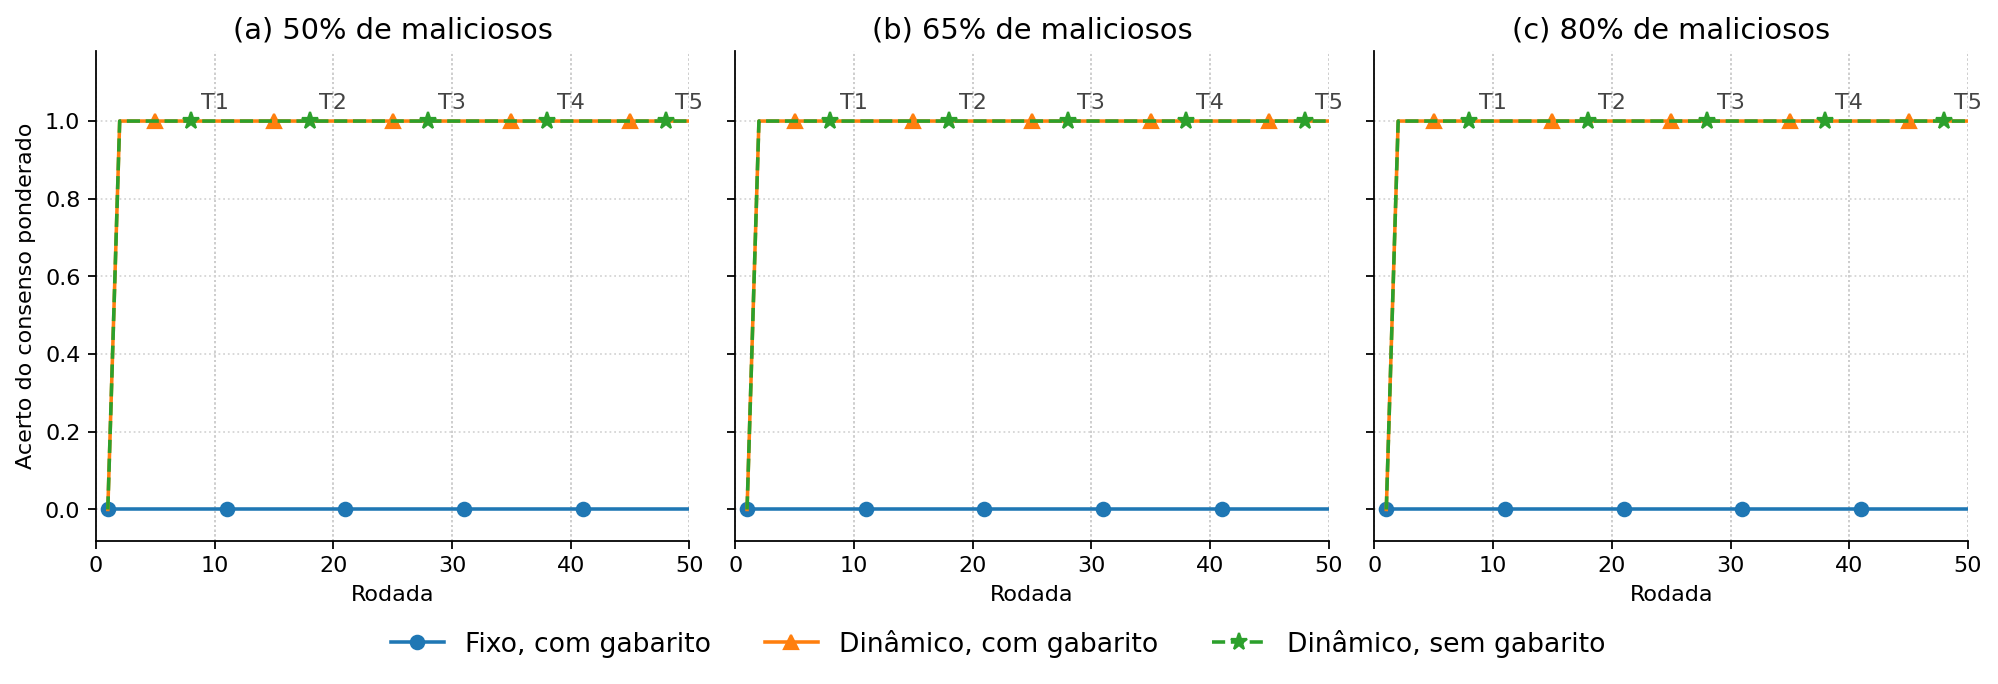
\includegraphics[width=0.92\textwidth]{figuras/acerto_por_rodada_50_65_80.png}
\caption{Acerto do consenso ponderado em cada rodada, pela Equação~\ref{eq:acerto-rodada}. Os painéis são 50\%, 65\% e 80\% de maliciosos. No dinâmico, as duas configurações coincidem a partir da segunda rodada. Em 65\%, o valor $1$ é a cópia dos 18 nós honestos; em 80\%, a dos 10.}
\label{fig:trajetoria}
\end{figure*}

Nesses três painéis, o fixo fica em $0$ da primeira à última rodada. A validação atualiza a reputação, e o consenso daquela rodada continua sendo $999$.

No dinâmico, a rodada 1 erra e, da rodada 2 em diante, o consenso ponderado acerta, com ou sem gabarito.

Em 50\% há uma cadeia só. Na primeira rodada todos têm reputação $0{,}5$, a soma total é $25$ e os 25 maliciosos confirmam $12{,}5$. Como o quórum pede estritamente mais da metade, a rodada forjada é anulada, e o líder e quem confirmou são punidos com $\alpha = 0{,}5$. Na configuração com gabarito a calibração ainda é aplicada depois da anulação: no início da rodada 2 cada malicioso está em $0{,}05$, a soma dos pesos de voto é $1{,}25$ para eles e, nas cinco repetições, ficou entre $17{,}7$ e $21{,}7$ para os honestos. Sem gabarito não há essa correção, e as somas são $6{,}25$ para os maliciosos e $12{,}5$ para os honestos. Nos dois casos a punição já separou as reputações por mais de $0{,}05$, o rodízio encerra, e o líder da rodada 2 é o honesto de menor identificador, \texttt{node-25}.

Em 65\% os 32 maliciosos confirmam $16$ de $25$, o quórum passa e o registro entra. Os 18 honestos recusam e seguem outra cópia. O consenso ponderado medido é o dessa cópia, que agrega só as respostas desses 18 nós; os 32 votos $999$ ficam na outra cópia e não entram nessa conta. A maioria simples continua sobre as 50 respostas, por isso fica em $0$. O valor $1$ do consenso ponderado e o valor $0$ da maioria simples saem de conjuntos diferentes de respostas, 18 nós na cópia honesta contra as 50 respostas da rede, e por isso essa comparação não contrapõe os dois agregadores sobre o mesmo conjunto. A configuração sem gabarito tem zero rodadas com gabarito e a mesma curva de acerto. Nas cinco repetições houve uma divisão e duas cadeias no fim.

Em 80\% os 40 maliciosos confirmam $20$ de $25$, o quórum passa e os 10 honestos recusam. O valor $1$ é a cópia desses 10 nós, e os 40 votos $999$ ficam na outra cópia. Nas cinco repetições, com e sem gabarito, houve uma divisão e duas cadeias no fim.

\subsection{Por que a validação não inverte o fixo}

A reputação média do perfil $P$ depois da rodada $t$, nas cinco repetições, é

\begin{equation}
\label{eq:rep-perfil}
\bar{R}_{P}^{(t)} = \frac{1}{|S|} \sum_{s \in S} \left( \frac{1}{|P|} \sum_{i \in P} R_i^{(t,s)} \right).
\end{equation}

A Figura~\ref{fig:reputacao} mostra essa média para o peso do voto no orquestrador dinâmico, em 50\% e em 80\% de maliciosos. Em 50\% há uma cadeia só. Em 80\% a rede se divide, e cada curva é a média na cópia em que o perfil ficou. Em 65\% as duas cópias não entram neste desenho.

\begin{figure*}[t]
\centering
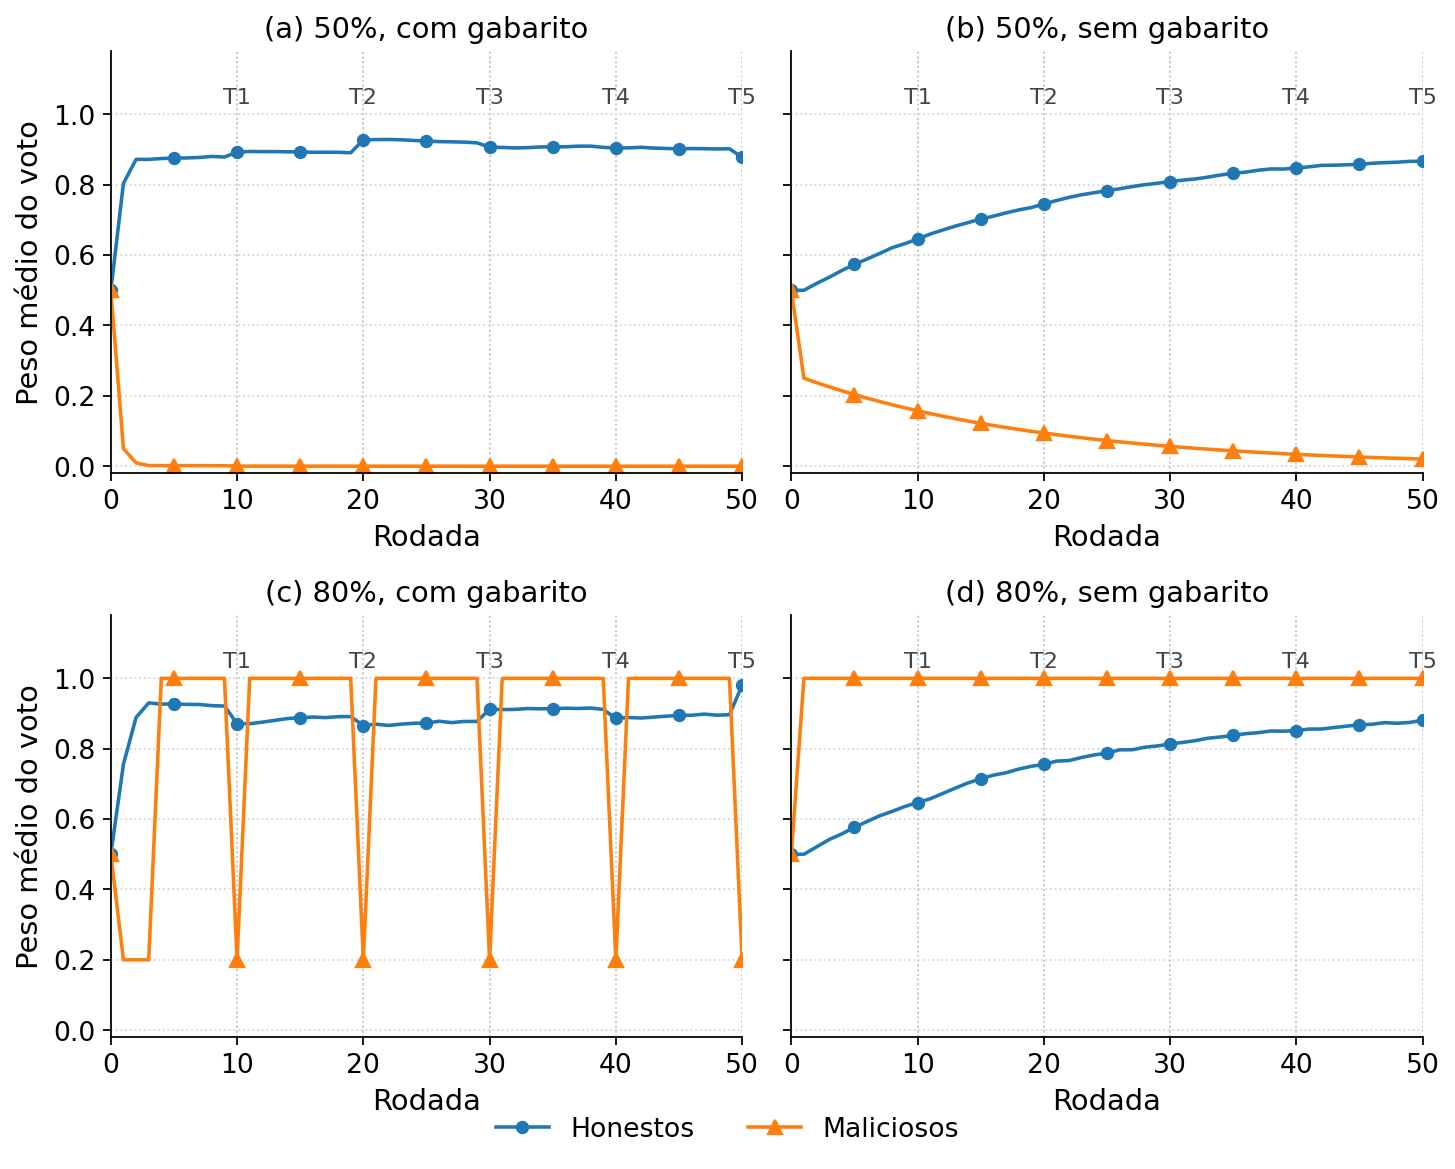
\includegraphics[width=0.92\textwidth]{figuras/reputacao_dinamico_50_e_80.png}
\caption{Peso médio do voto no orquestrador dinâmico, pela Equação~\ref{eq:rep-perfil}. Em cima, 50\% de maliciosos, uma cadeia só. Embaixo, 80\%: cada curva é a média na cópia do perfil, 40 maliciosos numa e 10 honestos na outra. Em 65\% as duas cópias não entram neste gráfico. As verticais são as rodadas 10, 20, 30, 40 e 50; com gabarito, são também a validação.}
\label{fig:reputacao}
\end{figure*}

No painel de 50\% com gabarito, a calibração separa os perfis na primeira rodada: a média das cinco repetições fica em $0{,}804$ para o honesto e em $0{,}050$ para o malicioso, e no fim da terceira rodada em $0{,}872$ e $0{,}002$. Sem gabarito, a punição deixa o malicioso em $0{,}250$ e o honesto em $0{,}500$; daí em diante só o peso do voto se move, com $\alpha = 0{,}05$, e na rodada 50 as médias são $0{,}867$ e $0{,}020$. A reputação de eleição, nesse caso, permanece em $0{,}25$. Em 80\%, com gabarito, a média dos honestos depois da primeira rodada fica em $0{,}756$, na cópia dos 10. Na cópia dos 40, o registro forjado grava peso $1$ para o conluio; nas rodadas com gabarito esse peso cai a $0{,}2$, com $s=0$ e $\alpha = 0{,}8$, e volta a $1$ na rodada seguinte. Sem gabarito, o malicioso permanece em $1$ nessa cópia e o honesto parte de $0{,}500$; na rodada 50 as médias são $0{,}881$ e $1$.

No orquestrador fixo, na rodada normal, o malicioso recebe $s=1$ e o honesto que não votou $999$ recebe $s=0$. Na validação, o malicioso recebe $s=0$ e o honesto que acerta o gabarito recebe $s=1$. O ciclo medido é de nove atualizações com um sinal e uma com o outro. Com $\alpha = 0{,}3$, $\beta = 1-\alpha = 0{,}7$ e $\gamma = \beta^{9}$, o valor logo depois da validação se repete:

\begin{equation}
\label{eq:ponto-fixo}
R_{m} = \frac{\beta(1-\gamma)}{1-\beta\gamma} = 0{,}691,
\qquad
R_{h} = \frac{\alpha}{1-\beta\gamma} = 0{,}309.
\end{equation}

$R_{m}$ é a reputação do malicioso. $R_{h}$ é a do honesto que discorda do consenso capturado nas nove rodadas e acerta a validação. No fixo, que não está nesta figura, a reputação média dos maliciosos cai em $0{,}686$ na rodada 10 e em $0{,}691$ nas rodadas 20, 30, 40 e 50, e sobe até $0{,}987$ antes da validação seguinte. A média dos honestos logo depois da validação fica em torno de $0{,}9 \times 0{,}309 \approx 0{,}278$, porque o honesto erra a validação com probabilidade $0{,}1$.

Logo depois da validação, o peso ainda está do lado do conluio. Em 50\%, $25 \times 0{,}691 = 17{,}3$ contra $25 \times 0{,}309 = 7{,}7$. Em 65\%, $32 \times 0{,}691 = 22{,}1$ contra $18 \times 0{,}309 = 5{,}6$. Em 80\%, $40 \times 0{,}691 = 27{,}6$ contra $10 \times 0{,}309 = 3{,}1$. A rodada seguinte devolve $s=1$ ao malicioso, e o dente de serra recomeça. Na configuração sem gabarito do dinâmico, o $1$ da Figura~\ref{fig:trajetoria} não vem dessas validações: essa configuração tem zero rodadas com gabarito.

Com $\alpha = 0{,}8$, a atualização é $R' = 0{,}2\,R + 0{,}8\,s$. Depois de uma rodada com gabarito, o honesto que acerta fica com reputação de pelo menos $0{,}8$ e o malicioso com no máximo $0{,}2$. Em 50\%, o conluio pesa no máximo $25 \times 0{,}2 = 5$, contra cerca de $0{,}9 \times 0{,}9 \times 25 \times 0{,}8 \approx 16$, dos cerca de 20 honestos que acertam a validação e a rodada seguinte. Em 65\%, o teto do conluio é $32 \times 0{,}2 = 6{,}4$, contra cerca de $0{,}81 \times 18 \times 0{,}8 \approx 11{,}7$. Em 80\%, o teto do conluio é $40 \times 0{,}2 = 8$, contra cerca de $0{,}81 \times 10 \times 0{,}8 \approx 6{,}5$. Essa conta não põe o honesto à frente, e o $1$ medido vem da divisão da cadeia. A diferença da Tabela~\ref{tab:teste} entre o fixo e o dinâmico com gabarito, portanto, não se explica só pelo orquestrador. A configuração sem gabarito isola a anulação, com a punição de quem confirmou, e a divisão da cadeia.

Na primeira rodada do fixo, em 50\%, todas as reputações valem $0{,}5$, então o ponderado coincide com a maioria, e o desempate dos dois é o menor valor. Se os 25 honestos acertam juntos, o que tem probabilidade $0{,}9^{25} \approx 0{,}072$, a rodada vai para o gabarito, o honesto sobe a $0{,}65$ e o malicioso cai a $0{,}35$, e o consenso permanece com os honestos. A chance de isso ocorrer em ao menos uma das cinco repetições é cerca de $0{,}31$, e não ocorreu: as cinco ficaram com acurácia de teste $0$. Em 65\% a conta não cabe, porque 32 votos iguais vencem os 18 honestos mesmo que todos acertem. Em 80\%, 40 votos iguais vencem os 10 honestos mesmo que todos acertem. Quem ganha a primeira rodada fica com a reputação, porque nas rodadas seguintes $s$ é a concordância com esse consenso.

% -----------------------------------------------------------
\section{Conclusão}
\label{sec:conclusao}

Em 50 nós e 50 rodadas, com maliciosos em conluio no valor $999$, a Rodada de Validação do orquestrador fixo, com $\alpha = 0{,}3$, não recupera o consenso ponderado quando o conluio tem 25, 32 ou 40 dos 50 nós. No orquestrador dinâmico, diante de um líder malicioso que forja o registro, a acurácia de teste chega a $1$ até $80\%$, por anulação de quórum em $50\%$ e pela cópia dos nós honestos em $65\%$ e em $80\%$, inclusive na configuração sem gabarito.

\begin{thebibliography}{Coulouris et al. 2021}

\bibitem[Hazarika and Shah 2024]{blockchainAI2024}
Hazarika, A. V. and Shah, M. (2024). Blockchain-based distributed AI models: Trust in AI model sharing. \textit{International Journal of Science and Research Archive}, 13(2):3493--3498. DOI: \url{https://doi.org/10.30574/ijsra.2024.13.2.2598}.

\bibitem[Bonawitz et al. 2019]{bonawitz2019}
Bonawitz, K. et al. (2019). Towards federated learning at scale: System design. In \textit{Proceedings of Machine Learning and Systems}.

\bibitem[Bouhata et al. 2025]{bouhata2025}
Bouhata, D., Moumen, H., Mazari, J. A., and Bounceur, A. (2025). Byzantine fault tolerance in distributed machine learning: a survey. \textit{Journal of Experimental \& Theoretical Artificial Intelligence}, 37(8):1331--1389. Publicado online em 2024. DOI: \url{https://doi.org/10.1080/0952813X.2024.2391778}.

\bibitem[Burns et al. 2022]{burns2022}
Burns, B., Beda, J., and Hightower, K. (2022). \textit{Kubernetes: Up and Running}. O'Reilly Media, Sebastopol, 3 edition.

\bibitem[Castro and Liskov 1999]{castro1999}
Castro, M. and Liskov, B. (1999). Practical Byzantine fault tolerance. In \textit{Proceedings of the Third Symposium on Operating Systems Design and Implementation (OSDI)}, pages 173--186, New Orleans. USENIX Association.

\bibitem[Chen et al. 2024]{chen2024}
Chen, W., Jia, L., Zhou, Y., and Ren, Q. (2024). Reputation-driven asynchronous federated learning for enhanced trajectory prediction with blockchain. \textit{arXiv preprint arXiv:2407.19428}.

\bibitem[Cobbe et al. 2021]{cobbe2021}
Cobbe, K., Kosaraju, V., Bavarian, M., et al. (2021). Training verifiers to solve math word problems. \textit{arXiv preprint arXiv:2110.14168}.

\bibitem[Coulouris et al. 2021]{coulouris2021}
Coulouris, G., Dollimore, J., Kindberg, T., and Blair, G. (2021). \textit{Distributed Systems: Concepts and Design}. Pearson, Boston, 6 edition.

\bibitem[Docker Inc. 2026]{docker2026}
Docker Inc. (2026). \textit{Docker Documentation}. Disponível em: \url{https://docs.docker.com}. Acesso em: 03 jun. 2026.

\bibitem[Kairouz et al. 2021]{kairouz2021}
Kairouz, P. et al. (2021). Advances and open problems in federated learning. \textit{Foundations and Trends in Machine Learning}, 14(1--2):1--210.

\bibitem[Kamvar et al. 2003]{kamvar2003}
Kamvar, S., Schlosser, M., and Garcia-Molina, H. (2003). The EigenTrust algorithm for reputation management in P2P networks. In \textit{Proceedings of the 12th International Conference on World Wide Web}.

\bibitem[Lamport et al. 1982]{lamport1982}
Lamport, L., Shostak, R., and Pease, M. (1982). The Byzantine generals problem. \textit{ACM Transactions on Programming Languages and Systems}, 4(3):382--401.

\bibitem[McMahan et al. 2017]{mcmahan2017}
McMahan, B. et al. (2017). Communication-efficient learning of deep networks from decentralized data. In \textit{Proceedings of the 20th International Conference on Artificial Intelligence and Statistics (AISTATS)}.

\bibitem[Russell and Norvig 2020]{russell2020}
Russell, S. and Norvig, P. (2020). \textit{Artificial Intelligence: A Modern Approach}. Pearson, Hoboken, 4 edition.

\bibitem[Shi et al. 2016]{shi2016}
Shi, W., Cao, J., Zhang, Q., Li, Y., and Xu, L. (2016). Edge computing: Vision and challenges. \textit{IEEE Internet of Things Journal}, 3(5):637--646.

\bibitem[Tanenbaum and van Steen 2017]{tanenbaum2017}
Tanenbaum, A. S. and van Steen, M. (2017). \textit{Distributed Systems}. Maarten van Steen, Amsterdam, 3 edition.

\bibitem[Wang et al. 2025]{wang2025}
Wang, B. et al. (2025). A decentralized asynchronous federated learning framework for edge devices. \textit{Future Generation Computer Systems}.

\bibitem[Wei and Liu 2025]{wei2025}
Wei, W. and Liu, L. (2025). Trustworthy distributed AI systems: Robustness, privacy, and governance. \textit{ACM Computing Surveys}, 57(6), Article 144, pages 1--42. DOI: \url{https://doi.org/10.1145/3645102}.

\bibitem[Wu et al. 2024]{wu2024}
Wu, H., Yue, C., Fan, Y., Li, Y., Flynn, D., and Zhang, L. (2024). Half a century of distributed Byzantine fault-tolerant consensus: Design principles and evolutionary pathways. \textit{arXiv preprint arXiv:2407.19863}.

\end{thebibliography}
\end{document}
